\documentclass[10pt,a4paper]{article}
\usepackage[utf8]{inputenc}

% Define the page margin
\usepackage[margin=3cm]{geometry}

% Better typography (font rendering)
\usepackage{microtype}

% Math environments and macros
\usepackage{amsmath}
\usepackage{amsfonts}
\usepackage{amssymb}
\usepackage{amsthm}

% Define \includegraphics to include graphics
\usepackage{graphicx}

% Draw graphics from a text description
\usepackage{tikz}

% Syntax highlighting
\usepackage{minted}

% Set global minted options
\setminted{linenos, autogobble, frame=lines, framesep=2mm}

% Import the comment environment for orgtbl-mode
\usepackage{comment}

% Do not indent paragraphs
\usepackage{parskip}

\title{Network Coding, Sheet 6}
\author{Marten Lienen (03670270)}

\DeclareMathOperator{\Null}{null}

\begin{document}

\maketitle

\section*{Exercise 1}

\subsection*{Part a)}

\begin{figure}[h]
  \centering
  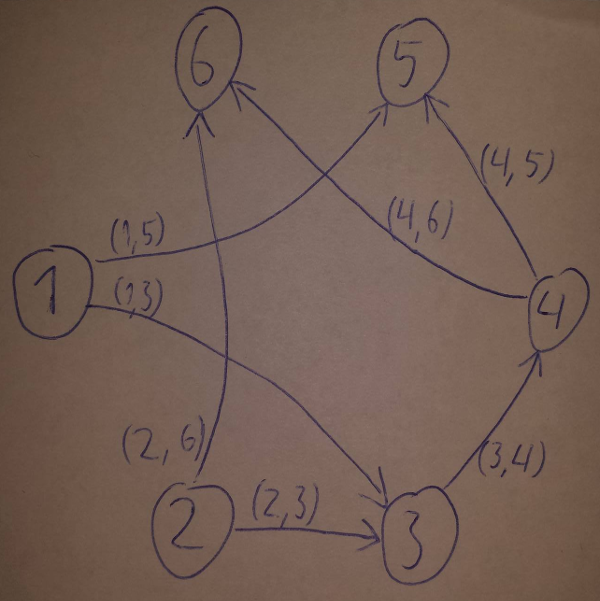
\includegraphics[width=\textwidth]{sheet-6/exercise-1-a}
  \caption{The network described by $M$}
\end{figure}

\subsection*{Part b)}

The rank is $6 - 1 = 5$ because it always equals the number of nodes minus $1$.

\subsection*{Part c)}

We know from the lecture that $\dim \Null M = 7 - 6 + 1 = 2$.
Therefore we have to look for two basis vectors, i.e. linearly independent undirected cycles.
\begin{equation*}
  B = \left\{
    \begin{pmatrix}
      1\\-1\\0\\0\\1\\1\\0
    \end{pmatrix},
    \begin{pmatrix}
      0\\0\\1\\-1\\1\\0\\1
    \end{pmatrix}
  \right\}
\end{equation*}

\subsection*{Part d)}

There is a $1$-$6$-cut $\{ (2, 3), (3, 4), (3, 5) \}$ of value $1$.
Since there is a connection between $1$ and $6$, this has to be a minimum and consequently the maximum flow.

\subsection*{Part e)}

\begin{equation*}
  r = \frac{d^{T}Mx}{|d|^{2}} = \frac{1}{|d|^{2}}d^{T}Mx
\end{equation*}

\subsection*{Part f)}

\begin{equation*}
  Mx = rd = \frac{1}{|d|^{2}}d^{T}Mxd = \frac{1}{|d|^{2}}dd^{T}Mx \Leftrightarrow \left( M - \frac{1}{|d|^{2}}dd^{T}M \right)x = 0 \Rightarrow B = M - \frac{1}{|d|^{2}}dd^{T}M
\end{equation*}

\subsection*{Part g)}

\begin{equation*}
  f = \left(\frac{d^{T}M}{|d|^{2}}\right)^{T} = \frac{1}{|d|^{2}}M^{T}d
\end{equation*}

\subsection*{Part h)}

\begin{align*}
  \min_{x} -\frac{1}{|d|^{2}}d^{T}Mx \text{ s.t. } 0 & = \left( M - \frac{1}{|d|^{2}}dd^{T}M \right)x\\
  x & \ge 0\\
  x & \le z
\end{align*}

The optimization program in figure \ref{fig:optimization-octave} written in octave finds the optimal flow
\begin{equation*}
  x = \begin{pmatrix}
    1 & 0 & 0 & 0 & 1 & 0 & 1
  \end{pmatrix}^{T}
\end{equation*}

\begin{figure}
  \inputminted{octave}{sheet-6/optimizeflow.m}
  \caption{Octave program for flow optimization}
  \label{fig:optimization-octave}
\end{figure}

\subsection*{Part i)}

\begin{equation*}
  Nx = Dr \Leftrightarrow r = (D^{T}D)^{-1}D^{T}Nx
\end{equation*}

\subsection*{Part j)}

\begin{equation*}
  Nx = Dr = D(D^{T}D)^{-1}D^{T}Nx \Leftrightarrow Nx - D(D^{T}D)^{-1}D^{T}Nx = 0 \Rightarrow B = N - D(D^{T}D)^{-1}D^{T}N
\end{equation*}

\subsection*{Part k)}

A has to be a matrix $A \in \mathbb{R}^{m \times 2m}$ that is composed of two concatenated identity matrices.
\begin{equation*}
  A = \begin{pmatrix}
    1 & \dots & 0 & 1 & \dots & 0\\
    \vdots & \ddots & \vdots & \vdots & \ddots & \vdots\\
    0 & \dots & 1 & 0 & \dots & 1
  \end{pmatrix}
\end{equation*}

\subsection*{Part l)}

\begin{align*}
  r = (D^{T}D)^{-1}D^{T}Nx & \Rightarrow r_{1} + r_{2} = \begin{pmatrix}1 & 1\end{pmatrix}r = \begin{pmatrix}1 & 1\end{pmatrix}(D^{T}D)^{-1}D^{T}Nx\\
                           & \Rightarrow f^{T} = \begin{pmatrix}1 & 1\end{pmatrix}(D^{T}D)^{-1}D^{T}N\\
                           & \Rightarrow f = \left( \begin{pmatrix}1 & 1\end{pmatrix}(D^{T}D)^{-1}D^{T}N \right)^{T}
\end{align*}

\subsection*{Part m)}

\begin{align*}
  \min -\begin{pmatrix}1 & 1\end{pmatrix}(D^{T}D)^{-1}D^{T}Nx \text{ s.t. } 0 & = (N - D(D^{T}D)^{-1}D^{T}N)x\\
  x & \ge 0\\
  Ax & \le z
\end{align*}

Interestingly octave is unable to optimize the flow in this situation and reports a zero-flow as the optimal solution.
Matlab on the other hand finds a real solution in the form of
\begin{equation*}
  x_{1} = \begin{pmatrix}
    0.7941\\
    2.0000\\
    0.0000\\
    0.0000\\
    0.7941\\
    0.7941\\
    0.0000
  \end{pmatrix}
  \qquad
  x_{2} = \begin{pmatrix}
    0.0000\\
    0.0000\\
    0.2059\\
    2.0000\\
    0.2059\\
    -0.0000\\
    0.2059
  \end{pmatrix}
\end{equation*}

\begin{figure}[h]
  \centering
  \inputminted{octave}{sheet-6/optimizeflow2.m}
  \caption{Octave program}
\end{figure}

\begin{figure}[h]
  \centering
  \inputminted{matlab}{sheet-6/optimizeflowmatlab.m}
  \caption{Matlab program}
\end{figure}

\subsection*{Part n)}

The maximum on the $r_{1}$-axis is $3$ because you can send $2$ directly and $1$ over node $3$.
The same is true of the $r_{2}$-axis since you can send $2$ packets directly and another one over node $3$.
Both flows share the edge $(3, 4)$ of capacity $1$.
So if one source starts to send over node $3$, the other has to lower its rate.
This suggests the achievable flow region sketched in figure \ref{fig:achievable-flow-region}.

\begin{figure}
  \centering
  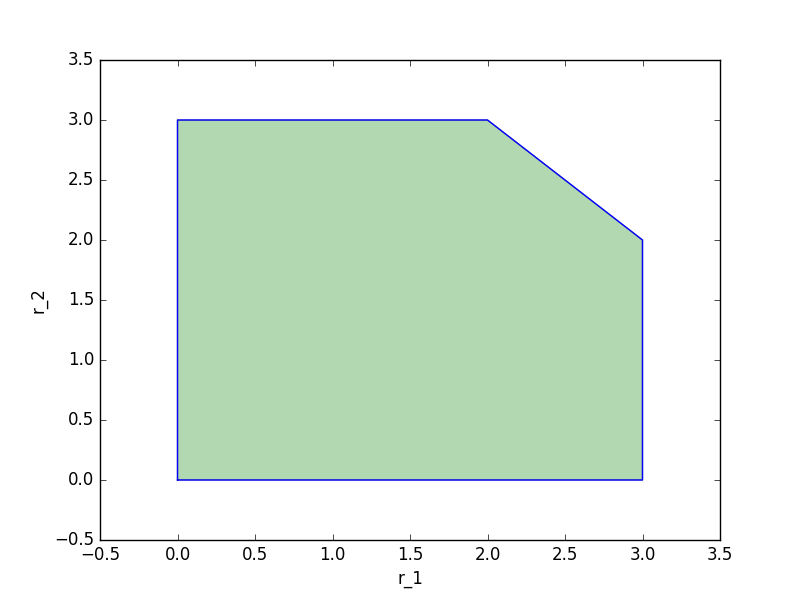
\includegraphics[width=\textwidth]{sheet-6/achievable-region.png}
  \caption{Achievable flow region}
  \label{fig:achievable-flow-region}
\end{figure}

\end{document}
